\let\negmedspace\undefined
\let\negthickspace\undefined
\documentclass[journal]{IEEEtran}
\usepackage[a5paper, margin=10mm, onecolumn]{geometry}
%\usepackage{lmodern} % Ensure lmodern is loaded for pdflatex
\usepackage{tfrupee} % Include tfrupee package

\setlength{\headheight}{1cm} % Set the height of the header box
\setlength{\headsep}{0mm}     % Set the distance between the header box and the top of the text

\usepackage{gvv-book}
\usepackage{gvv}
\usepackage{cite}
\usepackage{amsmath,amssymb,amsfonts,amsthm}
\usepackage{algorithmic}
\usepackage{graphicx}
\usepackage{textcomp}
\usepackage{xcolor}
\usepackage{txfonts}
\usepackage{listings}
\usepackage{enumitem}
\usepackage{mathtools}
\usepackage{gensymb}
\usepackage{comment}
\usepackage[breaklinks=true]{hyperref}
\usepackage{tkz-euclide} 
\usepackage{listings}
% \usepackage{gvv}                                        
\def\inputGnumericTable{}                                 
\usepackage[latin1]{inputenc}                                
\usepackage{color}                                            
\usepackage{array}                                            
\usepackage{longtable}                                       
\usepackage{calc}                                             
\usepackage{multirow}                                         
\usepackage{hhline}                                           
\usepackage{ifthen}                                           
\usepackage{lscape}
\begin{document}

\bibliographystyle{IEEEtran}
\vspace{3cm}

\title{1.4.6}
\author{EE24BTECH11058 - P.Shiny Diavajna}
% \maketitle
% \newpage
% \bigskip
{\let\newpage\relax\maketitle}

\renewcommand{\thefigure}{\theenumi}
\renewcommand{\thetable}{\theenumi}
\setlength{\intextsep}{10pt} % Space between text and floats


\numberwithin{equation}{enumi}
\numberwithin{figure}{enumi}
\renewcommand{\thetable}{\theenumi}

\textbf{Question:} If the point $\vec{P}\myvec{2 & 1}$ lies on the line segment joining points $\vec{A}\myvec{4 & 2}$ and $\vec{B}\myvec{8 & 4}$, then \\

   \solution
   \begin{table}[h!]    
     \centering
     \begin{tabular}[12pt]{ |c| c|}
    \hline
    \textbf{Variable} & \textbf{Description}\\ 
    \hline
	$\vec{P}\myvec{2 & 1}$ & Point on the linesegment joining $\vec{A}$ and $\vec{B}$ \\
    \hline 
	$\vec{A}\myvec{4 & 2}$ & one end of the linesegment $AB$ \\
    \hline
	$\vec{B}\myvec{8 & 4}$ & another end of the linesegment $AB$\\
    \hline 
    \end{tabular}

     \caption{Variables Used}
     \label{tab1.4.6.1}
   \end{table}


   \begin{align*}
      ||A-B||=\sqrt{(A-B)^\top(A-B)}\\
      \vec{A}=\myvec{4\\2}   \vec{B}=\myvec{8\\4}\\
      (A-B)=\myvec{-4\\-2}\\
      (A-B)^\top=\myvec{-4 -2}\\
   \end{align*}

   \begin{align*}
      AB=\sqrt{\myvec{-4 -2} \myvec{-4\\-2}} \\=2\sqrt{5}\\
   \end{align*}
   
   Similarly,

   \begin{align*}
      AP=\sqrt{\myvec{-2 -1} \myvec{-2\\-1}}\\=\sqrt{5}\\
      PB=\sqrt{\myvec{-6 -3} \myvec{-6\\-3}}\\=3\sqrt{5}\\
   \end{align*}

 Therefore,
   \begin{align*}
     AP=\frac{1}{2}AB
   \end{align*}

  \begin{figure}[h]
    \centering
    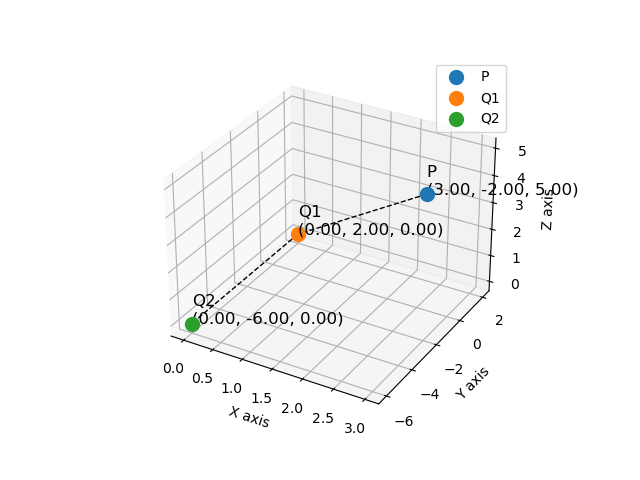
\includegraphics[width=\columnwidth]{/home/shiny/Desktop/mt/assignment2/figs/Figure_1.png}
    \caption{Plot of Points A, B and P}
 \end{figure}


\end{document}
